\documentclass[a4paper,11pt,twocolumn]{article}

\usepackage{icphs2023}
\usepackage{metalogo} % Only needed for the XeLaTeX logo
\usepackage{epstopdf}
\usepackage{tipa} %
\newcommand{\ipa}{\textipa}
\usepackage{amsmath}% http://ctan.org/pkg/amsmath
\newcommand{\argmax}{\mathop{\rm arg~max}\limits}
\newcommand{\argmin}{\mathop{\rm arg~min}\limits}
\usepackage{svg}

\hyphenpenalty=10000 % no hyphenation
% https://docs.google.com/document/d/1df4t0mZm1gUytgQOYaZNg6-mcneA4knqTvUPMIhoMMc/edit?usp=sharing
% https://docs.google.com/document/d/1VywiSaEORlVrRDb7nxGQx2D0pu6huftZrEiVQKmCGWY/edit?usp=sharing

\title{The role of allophones in phoneme perception models: Do devoiced vowels trigger vowel epenthesis?}
% \name{
\author{
    Takeshi Kishiyama$^1$,
    Chuyu Huang$^2$,
    Kei Furukawa$^3$,
    Yuki Hirose$^1$}
% \address{
\organization{
  $^1$Graduate School of Arts and Sciences, The University of Tokyo, Japan\\
  $^2$Faculty of Foreign Studies, Nagoya Gakuin University, Japan\\
  $^3$Nara Institute of Science and Technology, Japan}
\email{
    kishiyama.t@gmail.com,
    huang@ngu.ac.jp,
    furukawa.kei.fi4@is.naist.jp,
    hirose@boz.c.u-tokyo.ac.jp
    }
\begin{document}

\maketitle

\begin{abstract}
This study investigated how phoneme perception models should incorporate allophones, leveraging dialectical differences among Japanese in an AXB discrimination task. It has been reported that listeners of a language that does not accept consonant clusters insert epenthetic vowels, or illusory vowels, to repair illegal consonant clusters, thus, for example, perceiving VCCV as VCVCV. In addition to the roles of phonotactic constraints and acoustic cues, recent studies have indicated that allophones such as devoiced vowels also facilitate perceptual epenthesis. We compared the discrimination accuracies of VCCV and VCVCV perception in Tokyo and Kansai dialect speakers, who are reported to have less devoiced vowels. Both Tokyo and Kansai speakers perceived illusory vowels, indicating that illusory vowels were perceived even by speakers without the allophones. Furthermore, the results suggest that discriminative models other than probabilistic models assuming an auditory realization distribution can be psychologically valid.
\end{abstract}

\keywords{speech perception, phonotactics, context effects, perceptual epenthesis, dialect}

\section{Introduction}

When hearing speech that violates the phonotactics of the native language, the listener perceives the phonemes according to the rules. For example, native Japanese speakers perceive the speech [ebzo] as /ebuzo/ according to the phonotactics of their native language. The illusory vowel /u/ is supposed to be inserted and perceived for stimuli where the vocal fold vibration of the vowel is acoustically absent \cite{dupoux1999epentheticvi, dupoux2011illusory}. Through experiments on dialect speakers, this study reexamines the recently verified effects of allophones and discusses how we should incorporate them into perceptual models.

First, a large body of studies has reported the effect of phonotactics on vowel illusion \cite{dupoux1999epentheticvi, halle2014special, monahan2009not, mattingley2015influence, guevara2017predicting, guevara2017epenthetic}, as shown in an experiment with native French and Japanese speakers \cite{dupoux1999epentheticvi}. Unlike Japanese, French allows the consonant cluster /bz/, and the speakers of each language tried to discriminate between the sounds [ebuzo] and [ebzo] in the experiment. While French speakers were successful and did not perceive the vowel /u/ in [ebzo], Japanese speakers perceived [ebzo] as /ebuzo/, which decreased their discrimination accuracy.

Furthermore, experiments with native speakers of Brazilian Portuguese and Japanese have revealed the influence of acoustic cues on illusory vowels \cite{dupoux2011illusory}. Both languages do not allow /bz/, and the default vowels to be inserted are /i/ and /u/, respectively. The study deleted the vowels between /b/--/z/ in [ebizo] and [ebuzo], leaving the vowels' acoustic cues in /b/. As a result, the remained cues affected speakers of both languages, increasing the insertion rate of the non-default /i/ for native Japanese speakers. Therefore, acoustic cues influence which phoneme is activated.
These results made some research assume one-step models, where phonotactics and acoustic cues affect the illusion simultaneously. The one-step models can be represented by hidden Markov models (HMMs), which can also represent perceptual assimilation models \cite{best2001discrimination} and models in exemplar theory \cite{lacerda1995perceptual}, having reproduced the illusory vowels \cite{kishiyama2021influence} by calculating Equation 1. The equation calculates two likelihoods: $P(c|c_{t-1})$ represents the likelihood of the phoneme array $c_{t-1}$ to $c$, and $P(S_{\text{new}}|c)$ represents the likelihood of the input speech $S_{\text{new}}$ for all phonemes $c$. Consequently, the phoneme c that maximizes the likelihoods is activated as $\hat{c}$.

\begin{equation} \label{hmm}
    \hat{c} = \argmax_{c} P(c | c_{t-1})P(S_{\text{new}}|c)
\end{equation}

In the models above, acoustic cues such as coarticulation effects which phoneme would be activated. For example, the stimulus $S_{\text{new}}$ that contains the auditory feature of /i/ would make $P(S_{\text{new}}|\text{/i/})$ higher than $P(S_{\text{new}}|\text{/u/})$, changing the final $\hat{c}$. By contrast, allophones that belong to a single phoneme do not affect which phoneme to be activated because they are perceived as the same phoneme. Traditionally, the unit assumed as c above was phonemes \cite{wilson2013bayesian}, while two recent studies have suggested that allophones should be treated as discrete units in perceptual models.

First, it has been reported that devoiced or deleted allophones in Japanese better match to illegal consonant clusters, encouraging assimilation to the target phoneme and increasing the perceptual epenthesis \cite{kilpatrick2018japanese}. In Tokyo-dialect in Japanese, the high vowel /u/ in /esupo/ is deleted, and the auditory representation would be [espo] when it follows fricatives and affricates \cite{fujimoto2003devoice_eng, shaw2018lingual}. In other cases, the vowel in /epuso/ becomes devoiced as [ep\textsubring{\textturnm}so]. In the study, stimulus with those allophones increased the vowel illusion rate, indicating that the perceptual models should consider allophones explicitly. 

Furthermore, it has been reported that the transition probability between allophones causes vowel illusion \cite{kilpatrick2020japanese}. For example, in Japanese [\textctc], a realization of /s/ is more likely to be followed by /i/ compared to the other high vowels /u/. A previous study investigated whether [e\textctc{}po] induces the illusion of /i/ more \cite{kilpatrick2020japanese}, and they found that the /i/ was perceived more frequently after [\textctc] than after the baseline [g]. This result suggests that the transition probability between allophones affects the vowel illusion.

The question is whether phoneme perception models should consider these allophones as categorical realizations rather than as continuous acoustic features. Models without allophones, including the one-step models, can explain the results above. The difference in the auditory cues within the deleted and devoiced vowels can yield different probability in $P(S_{\text{new}}|c)$ in Eq. (1). Furthermore, the stimuli [\textctc] is supposed to share acoustic cues with /i/ \cite{kubozono1999japanese_eng}, which can also change $P(S_{\text{new}}|c)$ in Eq. (1) and the activation. To explain the results, therefore, the models do not need to have allophones.

One of the reasons why the above interpretations are possible for the experiments is the confounding of the allophones and the acoustic cues. First, in [ep\textsubring{\textturnm}so] and [espo], not only the allophonic vowels (devoiced or deleted) but also the immediately preceding speech sounds [p] and [s] are different, which makes it impossible to distinguish the effect of the categories from the acoustic features. In addition, even in comparisons such as [egpo] and [e\textctc{}po], the transition probability from [g] or [\textctc] to the following vowel is confounded with the acoustic information of [g] or [\textctc], so it is also impossible to distinguish whether the results are from the transition probabilities or not.

Therefore, the confounding needs to be resolved to discuss whether or not the deletion and devoicing should be considered a component of the model. We can leverage dialectal differences between the Kansai and Tokyo dialects in Japanese \cite{kishiyama2022onestep} to deal with this issue. The Kansai dialect speakers tend to devoice or delete vowels less frequently than the Tokyo dialect speakers do \cite{byun2011_eng, byun2012_eng}. According to the assumption that the deletion and devoicing caused the illusion, the Kansai-dialect speakers, who are also less exposed to those allophones, should yield fewer illusions and more accurate responses in discriminative AXB tasks.

\section{Perception experiment}

The perceptual task examines how devoicing and deletion increase the illusion. If deletion or devoicing vowels increase the perceptual illusion, the discrimination accuracy in the AXB task would be lower for Tokyo dialect speakers, who have more frequent contact with the variation. The opposite pattern is expected among the Kinki dialect speakers, who have less frequent or don't have contact with those.

\subsection{Materials and methods}

%FIXME: 分布の図なんて入れる余裕ない
We used an outsourcing service to recruit subjects who were older than 18 years. We set the subjects' residence to be Tokyo or the Kansai region, and those who had never lived in other areas since birth had priority in the recruitment process. In the end, 62 valid subjects participated in the experiment (M=40, SD=15). Figure 1 shows the distribution of age and residence history in the Kansai and Tokyo regions on the horizontal axis. Sixty-two subjects participated, but the results of the four subjects whose answers were under 75\% accuracy in the categorization task (\S3) were excluded from the analysis.

In the AXB task, the participants were asked to distinguish between VC$_\text{1}$VC2V and VC$_\text{1}$C2V patterns. To create an environment in C$_\text{1}$C$_\text{2}$ where deletion and devoicing occur, we established four pairs for C$_\text{1}$C$_\text{2}$: s--p, k--t, p--s, and ts--k. Although these consonant pairs are different from previous studies \cite{kilpatrick2018japanese}, we prepared these pairs for generalizing the results. In addition, we also designed a stimulus VC$_\text{1}$VC$_\text{2}$V with /u/ between C$_\text{1}$C$_\text{2}$ to have participants discriminate it from VC$_\text{1}$C$_\text{2}$V.

We also created two patterns depending on whether a trial's stimulus in the X position was either VC$_\text{1}$VC$_\text{2}$V or VC$_\text{1}$C$_\text{2}$V, which is to be distinguished in the AXB task. In addition, we prepared voiced counterparts of C$_\text{1}$ and C$_\text{2}$, such as b--z, where neither deletion nor devoicing occurs. The positions of correct answers were counterbalanced, A or B. Therefore, a list of target stimuli included 32 items based on the combination of the four conditions above. The 32 items were randomized and presented to each subject with 24 filler items.

We recorded stimuli from three male speakers and adjusted the loudness to around 75 dB. The duration before C2 was adjusted to about 50 ms (about 400 ms for the entire three moras) so that the subjects would not insert the "geminate" consonant (a distinctive phoneme sokuon in Japanese) in a long blank. We removed the voicing parts of /egudo/ and /ebuzo/based on formant and power and extended the silent interval. In this case, the cycle of each preceding waveform was duplicated and extended. In contrast, /u/ in /epuso/ was cut so that it would be of the same duration as /epuso/.

After three sets of practice tasks, 32 items were randomized and presented to the subjects in an experimental environment conducted on web browsers. A "+" was introduced in the center of the screen for 1000 ms before the audio stimuli, and the three audio items were presented at intervals of 200 ms. After the presentation was over, the subject was to respond as quickly as possible. We didn't feed back correct or incorrect to avoid learning during the task, and the program only provided answers in the practice task. When a trial ended, the participants could start the subsequent trial by pressing the space key.

\subsection{Results}

The results of the experiment are shown in Figure \ref{fig:axb_results}. The vertical axis shows the average discrimination accuracy of VC$_\text{1}$VC$_\text{2}$V and VC$_\text{1}$C$_\text{2}$V in the AXB discrimination task. On the left and right sides, we indicated whether the stimulus was in devoicing environment (e.g., k--t if C$_\text{1}$C$_\text{2}$ was devoicing condition, g--d if not). The horizontal axis shows the Tokyo--Kansai ratio, the ratio of residential history between Tokyo and the Kansai region. For example, if a subject has lived in Tokyo for 25 years and in Kansai for 15 years, the ratio is $(25-15)/40$, or $0.25$. We showed four items vertically to see tendencies for each item,

% FIXME: caption変更
\begin{figure}[!ht]
\begin{center}
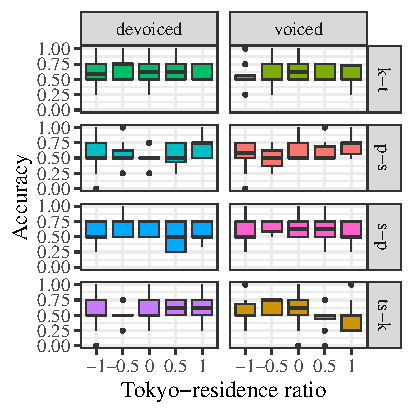
\includegraphics[width=7cm]{../results/artifact/results_axb_allophone.pdf}
\caption{The vowel chart used in the International Phonetic
Alphabet (IPA).}\label{fig:axb_results}
\end{center}
\end{figure}


We checked the distribution of the reaction time data and excluded the 1\% of data with a reaction time of 10 seconds or longer as outliers. We calculated the average accuracy based on the X in AXB (VC$_\text{1}$VC$_\text{2}$V or VC$_\text{1}$C$_\text{2}$V) and the correct answer position (A or B), reducing the data amount to 1/4. In doing so, we excluded missing values. The dependent variable was the average of correct and incorrect answers.

We created a Bayesian linear mixed-effects model \cite{lme4, rstanarm, easystats} with the Tokyo--Kansai ratio as the independent variable and the AXB task discrimination accuracy as the dependent variable. Item type and subjects were added as random effects. The analysis revealed an overall mean accuracy of 0.59, with no consistent effect for environmental or dialectal differences. The estimates were also positive and not in the direction of decreasing precision (Table 1).

Although we found no effect for the presence or absence of the residence ratio, a Bayes factor for the Tokyo--Kansai ratio was calculated to evaluate the null hypothesis. The Bayes factor was 0.150, providing substantial evidence for the null hypothesis. In the framework of Bayesian statistics, the Bayes factor is used as a decision-making index when comparing and discussing the effects of models and factors. Bayes factor can be derived in several ways, but in this study, we used as following.

$BF = Posterior Odds / Prior Odds$

Each $Odds$ above calculates the ratio of (i) the probability of the factor's effect to (ii) the probability supporting the null effect. This time, the factor was the Tokyo--Kansai ratio, an independent variable whose effect was supposed to be negative. Therefore, the \textit{null region} (Kruschke, 2010), considered to have no effect, was set to a positive value [0, Inf]. The probability of effect is the probability that slope $b$ falls outside the \textit{null region}. In contrast, the probability of no effect is the probability that it falls within the region. The $Prior Odds$ is calculated based on the prior distribution, whereas $Posterior Odds$ is calculated based on the observed data.

$Prior  Odds = P(b\notin[0, Inf]) / P(b\in[0, Inf])$

$Posterior Odds = P(b\notin[0, Inf] | Data) / P(b\in[0, Inf] | Data)$

The BF of the Tokyo--Kansai ratio was 0.15 when the null region was set to [0, Inf] in this analysis, which could indicate that the null hypothesis of a positive effect is 1/0.15, or about 6.67 times more plausible than the alternative hypothesis of a negative effect. This result contradicts the interpretation that the allophone increases the rate of illusions and reduces the accuracy.

\subsection{Discussion}

This study discusses whether models of phoneme perception should incorporate devoicing and deletion. If the allophone creates the illusion of a vowel, the Tokyo dialect speakers with the allophone should have lower accuracy in the discrimination experiment than speakers without devoicing. However, the results of the AXB task showed that the discrimination accuracy of both Kansai and Tokyo dialect speakers, regardless of their language experience, was around 0.59, which is close to a chance level. In addition, the Bayes factor values suggested that the language experience did not affect the rate of illusions in the discrimination task. Thus, we suggested that the presence or absence of an unusual sound did not cause the illusion.

Next, we conducted an offline categorization task to confirm that Kansai dialect speakers perceive the stimuli the same way as Tokyo dialect speakers. This experiment provides information on the acceptabilities of the stimuli and the subject's rate of correct responses to the task. It also provides an offline evaluation of the illusion.


\section{Categorization task}

The categorization task investigated dialectal differences and acceptability judgments about devoicing in offline processing. We examined whether dialect differences in language experience affect the goodness rating of deletion/devoicing. Note that we performed this categorization assignment after the online process to avoid any effect on the validation of the online process.

\subsection{Materials and methods}

The same subjects participated in the perceptual task. All speech sounds presented in the perceptual experiment were to be classified. There are a total of eight different patterns: four environments to be devoiced in the Tokyo dialect (esupo, ekuto, epuso, etsuko) and four devoiced settings (espo, ekto, epso, etsko). The choices were shown in Japanese letters on the screen, and the correct ones were esupo, ekuto, epuso, and etsuko, respectively. The environment where devoicing does not occur is one in which each of the above eight patterns of consonants is switched to voiced sounds, and the correct responses are ezubo, egudo, ebuzo, and edzugo, respectively. Since three speakers recorded 16 patterns, the subjects heard 48 stimuli.

Subjects listened to the stimuli, selected which of the above eight options shown above was closest to it, and immediately rated its acceptability on a 7-point scale (0--6). In the goodness of fit rating, zero was considered "not appropriate at all," and six was considered "completely appropriate."

\subsection{Results}

In analyzing the categorization results, Figure \ref{fig:cat_results} shows the Tokyo-Kansai ratio on the X-axis and the goodness of fit rating on the Y-axis in a boxplot. The left and right panes indicate the environment of speech (devoicing or not), and the color difference is shown in blue when the actual stimulus was devoiced and in red when it is not.

% FIXME: caption変更
\begin{figure}[!ht]
\begin{center}
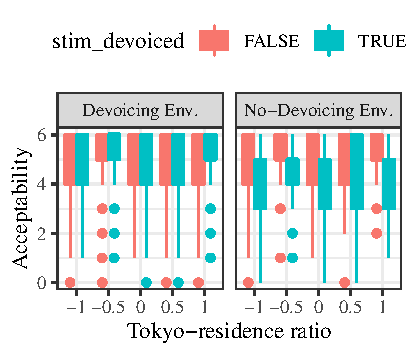
\includegraphics[width=7cm]{../results/artifact/results_categorization.pdf}
\caption{The vowel chart used in the International Phonetic
Alphabet (IPA).}\label{fig:cat_results}
\end{center}
\end{figure}

Figure X shows that overall ratings are above the mean of 3. In the left pane, which represents the devoiced environment, the ratings of the devoiced stimulus were higher, as shown in blue. In contrast, the right pane, which represents the no-devoicing environment, suggests the devoiced stimulus decreased the ratings. Residential history does not contribute to these differences.

To test these points, we created a Bayesian linear mixed-effects model with the goodness of fit rating as the dependent variable. Five independent variables were environment (devoicing/no-devoicing), stimulus type (devoiced / not devoiced), the Tokyo--Kansai ratio, an interaction between the three variables, an interaction between environment and stimulus, and an interaction of the three factors. Subjects and items were random effects. As a prior distribution for each parameter, we employed a normal distribution with a mean of 0 and a standard deviation of 10, which we consider a uniform distribution with a sufficiently wide range. Table X below shows the coefficients, sd, and 95\% Bayesian confidence intervals for each factor obtained by MCMC sampling. All Rhat values were one, and the model converged.

Below is the table which summarizes statistics whose 95\% Bayesian confidence interval did not include 0. First, the mean rating was 4.87, indicating that the evaluation was generally natural, given that the rating range was 0--6. The devoicing environment and the devoiced stimulus were $-0.37$ and $-0.79$, respectively. Furthermore, the interaction, i.e., the devoiced stimulus in the devoiced environment, increased the rating by 1.19. The BF for the Tokyo--Kansai ratio was 0.012 when the null region was set to $[-\inf, 0]$, indicating robust evidence of no effect.

\subsection{Discussion}

The results showed that the overall responses were above 4, which means that the quality of the stimuli in this study was not lower than in previous studies \cite{kilpatrick2018japanese}. If the subjects can judge the devoiced speech in the Tokyo dialect offline without epenthesis, then the goodness rate of devoiced stimuli would be above three because it is appropriate in devoicing environment and less than three if it is in a no-devoicing environment. In contrast, when vowels are inserted, all are appropriate and acceptable; thus, responses would be above 4.

The results of the categorization task showed that both Tokyo dialect and Kansai dialect speakers showed higher ratings when the environment and speech were in the Tokyo dialect. In other words, the results showed that the rating increased when the speech was devoiced in a devoicing environment. At the same time, it decreased when the devoiced stimuli were in the no-devoicing environment. However, the effect was only about 1, not high enough to cross the threshold between unnatural and natural.

\section{General Discussion}

Previous research proposed that the vowel illusion was caused by devoicing. In addition, probabilistic models included the distribution of auditory realizations. This study proposes a different interpretation based on the results of perceptual experiments and categorization tasks.

First, the results of the discrimination accuracy and categorization tasks in the previous studies were not due to the effect of devoicing but to acoustic differences. Suppose the perceptual epenthesis was due to the devoicing or deletion. In that case, the discrimination accuracy of Tokyo dialect speakers should be lower than that of Kansai dialect speakers who do not devoice or delete the vowels, but there was no such effect. Instead, the Kansai dialect speakers perceived the illusory vowels as the Tokyo dialect speakers do in our study.

Second, regarding how acoustic cues affect speech perception, previous studies \cite{wilson2013bayesian, kishiyama2021influence} have assumed Eq. \ref{hmm} during inference. On the right-hand side, $P(S_{\text{new}}|c)$ is thought to represent the distribution of auditory realizations for phonemes or the perceptual likelihood of $S_{\text{new}}$ given $c$. This formula makes the results consistent with the previous study because $P$( [\textsubring{\textturnm}] | /u/ ) or $P$( [s] | /su/ ) is not zero given that the Kinki dialect speakers hear them since these are in Tokyo-dialect, which are prevalent in Japan. Given Bayes Theorem, however, the equation can be rewritten as Eq. (\ref{disc}).

% cˆ = argmax c P(c|ct−1) (P(c |Snew )/P(c))
% FIXME: ここの修正
\begin{equation} \label{disc}
    \hat{c} = \argmax_{c} P(c | c_{t-1}) \frac{P(c|S_{\text{new}})}{P(c)}
\end{equation}

The equation above implies that the above equation integrates a discriminative model rather than a generative model with the auditory distribution. Thus, it can employ other discriminative models, such as neural networks and multinomial logistic regressions. Since previous studies have already supported the validity of HMM \cite{kishiyama2021influence}, we will test whether we can incorporate the above discriminative model into HSMM to explain behavioral data.

\bibliographystyle{IEEEtran}

\bibliography{mybib}

\end{document}
